
\begin{figure}
	\centering
	\begin{subfigure}{\columnwidth}
		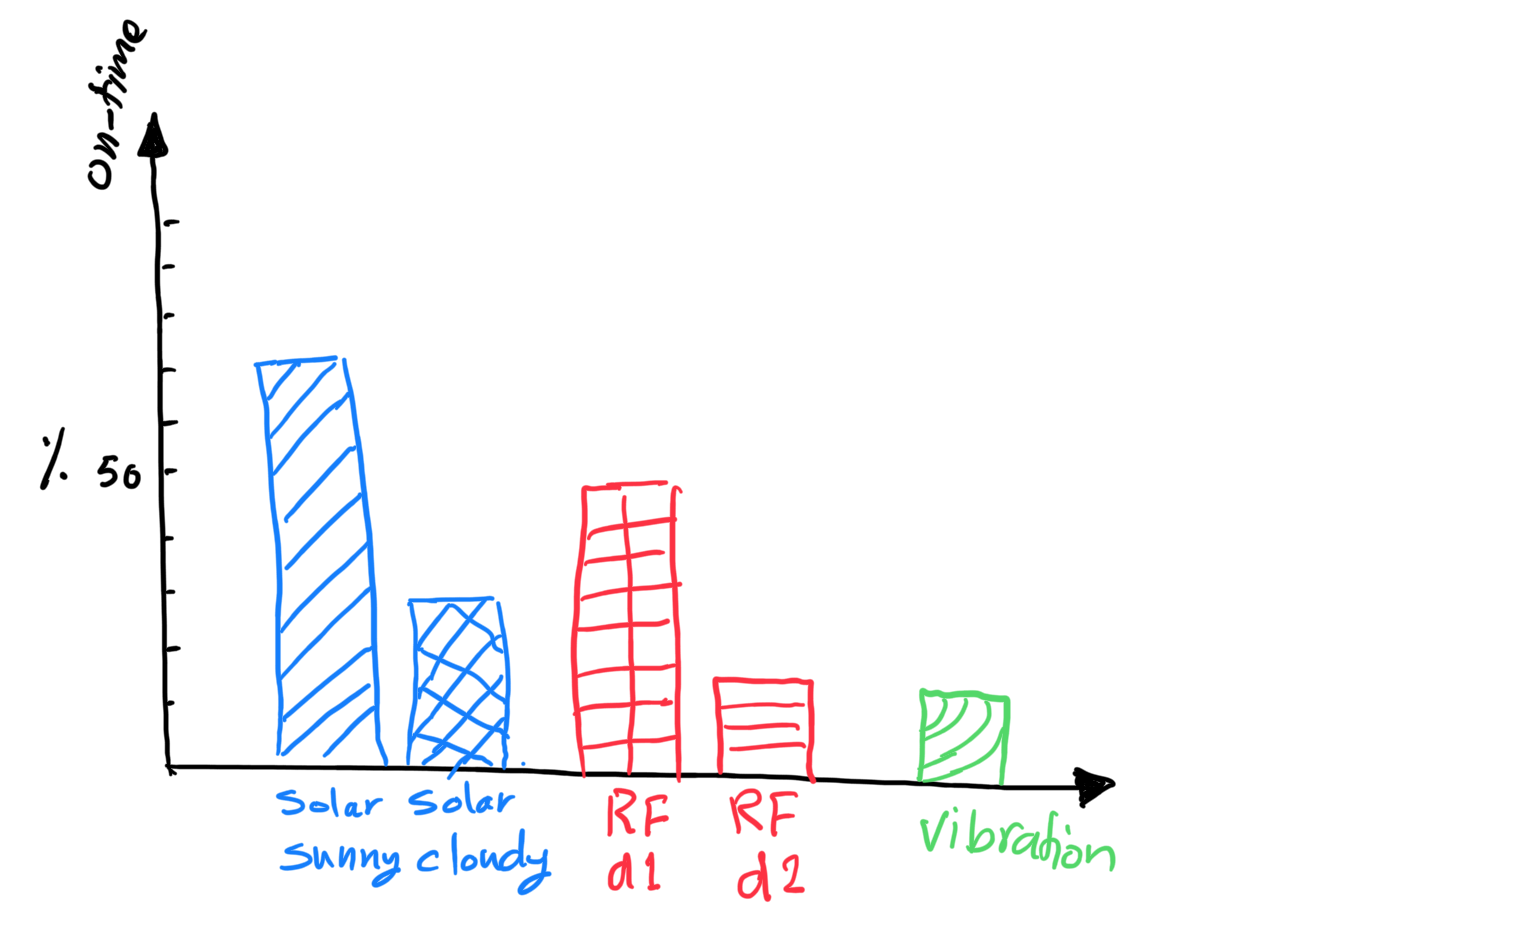
\includegraphics[width=\columnwidth]{figures/intermittent_problem}
		\caption{The on-time percentage of an intermittent device powered by different energy sources relative to its on/off cycle length}
		\label{fig:disInterSys}
	\end{subfigure}
	\begin{subfigure}{\columnwidth}
		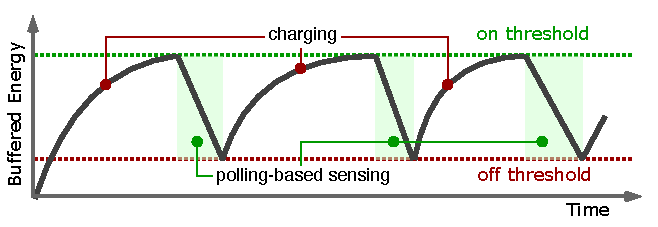
\includegraphics[width=\columnwidth]{figures/PowerCycleIntermittentSystem}
		\caption{The power cycle of an intermittently powered device.}
		\label{fig:powerCycle}
	\end{subfigure}
\end{figure}

Intermittently powered devices use their environment as an energy source instead of batteries. Therefore, they promise a small, cheap, and maintenance-free version of the current Internet of Things (IoT) edge devices. Driven by this vision, recent years have paid significant attention to intermittent systems~\cite{hicks2017clank,lucia2017intermittent,colin2016chain,colin2018termination,yildirim2018ink}. 
%
%%% knowledge gap, unknown information
However, their inherent sporadic operation patterns (Figure~\ref{fig:disInterSys}) have prevented researchers from demonstrating real word applications, for example \cite{colin2016chain,hester2017timely} present activity recognition applications without driving a real sensor to capture external signals.

%
%%% Hypothesis, question, purpose statement
This paper responds to the challenge of intermittent power supply by introducing the concept of \textit{distributed intermittent systems}. A distributed intermittent system is defined as the abstraction of a group of tiny intermittently powered devices (or nodes). The on-time of the distributed intermittent system should approach continuous time as the number of intermittent devices increases. However, the on-time and off-time of  distributed intermittent systems depend on the environment and the load. As such, we do not expect, for example, a linear relationship between the number of nodes and the overall on-time.

Controlling the on/off cycle of intermittent devices enables adapting them to many real world applications. For example, once a certain on/off cycle is preserved, an intermittent wake-up receiver can be implemented; intermittent acoustic monitoring system for monitoring engines modules---the sound produced by a deformed gear tooth---can be made. Moreover, with the advances in passive communication (such as passive light~\cite{}, and backscatter tag-to-tag~\cite{} communication) battery-free miniaturized sensors can form self-powered wireless sensor network to, for instance, create smart wallpaper and revolutionize smart buildings. 


This paper pushes the boundaries of intermittent systems by:
\todo{update the contributions and challenges}
\begin{itemize}
		\item introducing \textit{distributed intermittent systems} to control the duration of the up time of intermittent sensors and increase their responsiveness,
		\item investigating the relation between distributed intermittent systems power cycle and their environment,
		\item demonstrating the \textit{world's first} distributed intermittent system: a distributed microphone. 
\end{itemize}
%\todo{add the challenges and contributions}
%%% Approach, plan of attack, proposed solution



